\section{Q3: Autoencoders}
\label{sec:q3}

\subsection{(a) Bottleneck capacity}
The three convolutional autoencoders share everything except the bottleneck. The encoder is three stride-2
$4\times4$ convolutions (32, 64, 128 channels, BatchNorm, ReLU) down to $128\times4\times4$ followed by a linear
layer to a $d$-dimensional code; the decoder mirrors it with transposed convolutions. Only the two linear
layers change with $d \in \{16, 128, 1024\}$ (192$\times$, 24$\times$ and 3$\times$ compression of the 3072
input values). All three are trained identically without labels: AdamW (lr $10^{-3}$, weight decay
$10^{-5}$), OneCycle, 30 epochs, batch 256, MSE in the normalised input space, seed 242003. Working in the
normalised space lets reconstructions go straight into the Q1 classifier; errors are also reported in $[0,1]$
pixel units.

\begin{table}[t]
\centering
\small
\begin{tabular}{@{}rrcc@{}}
\toprule
$d$ & Params & Val MSE (norm.) & Val MSE (pixel) \\
\midrule
16 & 398{,}995 & 0.2633 & 0.01650 \\
128 & 857{,}859 & 0.0800 & 0.00502 \\
1024 & 4{,}528{,}771 & 0.0308 & \textbf{0.00194} \\
\bottomrule
\end{tabular}
\caption{Q3(a). Validation reconstruction error after 30 epochs. Selected: $d=1024$; its test MSE is 0.00194
(pixel), PSNR 27.1\,dB.}
\label{tab:q3a}
\end{table}

If reconstruction error is the only criterion there is no trade-off to make: validation error falls steadily
with $d$ (Tab.~\ref{tab:q3a}), so $d=1024$ is selected. Its test error (0.00194) equals its validation error,
so the choice did not overfit the validation split. It is still far from an identity map: fine texture and
sharp edges are smoothed (Fig.~\ref{fig:q3rec}, row 4).

\begin{figure}[t]
\centering
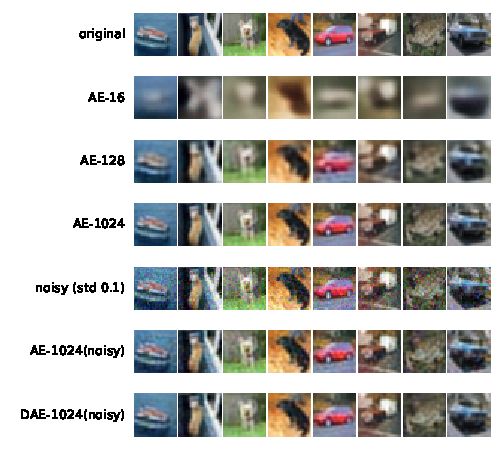
\includegraphics[width=\columnwidth]{q3_reconstructions}
\caption{Q3. Test images and their reconstructions by the three clean autoencoders, the noisy input
($\sigma=0.1$), and the clean AE and the DAE applied to the noisy input.}
\label{fig:q3rec}
\end{figure}

\subsection{(b) Does denoising recover what the classifier needs?}
\textbf{Corruption and protocol.} Additive Gaussian noise with standard deviation $\sigma=0.1$ in $[0,1]$ pixel
units, clipped to $[0,1]$. Reconstruction can reasonably help here because the noise is independent per pixel
while natural images are smooth and correlated (unlike occlusion or blur, which remove information that can only
be guessed). The denoising autoencoder (DAE)~\cite{vincent2008extracting} has the same architecture and
bottleneck as the selected clean AE and the same optimiser, schedule and epochs; its input is a noisy image
(noise redrawn every batch) and its target the clean image. No labels are used. The classifier is the selected
Q1(a) CNN (test accuracy 0.897), kept fixed. Test noise is drawn once with a fixed seed; we also report
$\sigma=0.05$ and $0.2$, and the classifier on reconstructions of \emph{clean} images as a control.

\begin{table}[t]
\centering
\small
\begin{tabular}{@{}lccc@{}}
\toprule
Classifier input & $\sigma=0.05$ & $\sigma=0.1$ (train) & $\sigma=0.2$ \\
\midrule
Noisy image & \textbf{0.655} & 0.280 & 0.115 \\
Clean AE (noisy) & 0.616 & \textbf{0.553} & 0.406 \\
DAE (noisy) & 0.548 & 0.524 & \textbf{0.422} \\
\midrule
\multicolumn{4}{@{}l}{Control, no noise: clean image 0.897; clean AE 0.646; DAE 0.553} \\
\multicolumn{4}{@{}l}{MSE to clean at $\sigma=0.1$: noisy 0.0093, AE 0.0032, DAE 0.0030} \\
\bottomrule
\end{tabular}
\caption{Q3(b). Test accuracy of the fixed Q1(a) CNN.}
\label{tab:q3b}
\end{table}

\textbf{Result.} At the trained noise level the DAE brings the classifier from 0.280 back to 0.524
(Tab.~\ref{tab:q3b}), so it recovers a large part of what the noise destroyed, but nowhere near the clean
0.897. The control rows explain why: a \emph{clean} image passed through the clean AE already drops to 0.646, and
through the DAE to 0.553. Both autoencoders keep layout and colour but remove texture and edges the CNN relies
on, so about 0.65 is a ceiling for reconstruct-then-classify with these models. Two further observations show
that pixel error is the wrong yardstick. The DAE's outputs are closer to the clean images in MSE than the clean
AE's (0.0030 vs 0.0032) yet give lower accuracy (0.524 vs 0.553): it smooths more aggressively, which lowers MSE
against noise and also removes texture. And the DAE is the best option only at the stronger noise $\sigma=0.2$;
at $\sigma=0.05$ the noisy image itself is better than either reconstruction. Our answer is therefore that
denoising recovers \emph{some} class information (+24 points) but not the information the classifier needs to
approach its clean accuracy, because the reconstruction step removes it. Part of the loss is a distribution
shift for a classifier trained on sharp images; retraining it on reconstructions would be a different experiment
and is excluded by the question.

\subsection{(c) Class information vs reconstruction quality}
The encoders are frozen and their bottleneck codes are probed in two ways: a multinomial logistic regression
(features standardised with train statistics, L2 weight in $\{10^{-5},\dots,10^{-1}\}$ chosen on validation) and
a cosine $k$-NN ($k\in\{1,\dots,100\}$ chosen on validation). Raw pixels are included as a reference.

\begin{table}[t]
\centering
\small
\begin{tabular}{@{}lccccc@{}}
\toprule
Code & Dim & MSE (px) & PSNR & Linear & $k$-NN \\
\midrule
AE-16 & 16 & 0.0165 & 17.8 & 0.331 & 0.422 \\
AE-128 & 128 & 0.0050 & 23.0 & 0.410 & 0.409 \\
AE-1024 & 1024 & \textbf{0.0019} & \textbf{27.1} & 0.532 & 0.485 \\
DAE-1024 & 1024 & 0.0024 & 26.1 & \textbf{0.550} & \textbf{0.490} \\
Raw pixels & 3072 & -- & -- & 0.415 & 0.426 \\
\bottomrule
\end{tabular}
\caption{Q3(c). Test reconstruction error of clean images and test accuracy of probes on frozen codes.}
\label{tab:q3c}
\end{table}

\begin{figure}[t]
\centering
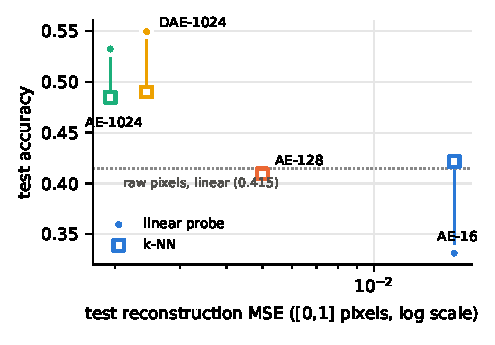
\includegraphics[width=0.9\columnwidth]{q3_recon_vs_probe}
\caption{Q3(c). Reconstruction error (log) against test accuracy of a linear probe (dots) and $k$-NN (squares)
on the frozen code. The two AE-128 markers overlap (0.410 / 0.409).}
\label{fig:q3c}
\end{figure}

Across the three clean autoencoders, better reconstruction goes with more linearly available class information
(0.331, 0.410, 0.532), so at a coarse level the two agree (Tab.~\ref{tab:q3c}, Fig.~\ref{fig:q3c}). They part
ways in two places. The DAE reconstructs clean images worse than AE-1024 but its code holds more class
information (0.550 vs 0.532 linear; the $k$-NN gap of 0.5 points is within single-seed noise). A plausible reason
is that removing noise forces the code to keep structure that is stable under small pixel changes, which is more
related to the class than exact pixel values. Second, under $k$-NN the 16-d code (0.422) beats the 128-d code
(0.409) despite three times the reconstruction error, while the linear probe ranks them the other way. Moreover,
AE-128 is no better than raw pixels at all. We conclude that the two quantities agree only roughly and that
reconstruction error is not a reliable proxy for how useful a representation is for classification.
